\documentclass[10pt,a4paper]{article}
\usepackage[utf8]{inputenc}
\usepackage[spanish]{babel}
\usepackage{amsmath}
\usepackage{amsfonts}
\usepackage{amssymb}
\usepackage{graphicx}
\usepackage[left=2cm,right=2cm,top=2cm,bottom=2cm]{geometry}
\usepackage[hidelinks]{hyperref}
\usepackage{listings}
\lstset{     frame = single,     framexleftmargin = 15pt }
\begin{document}

\begin{titlepage}
\title{\textbf{{\Huge Práctica 1 - Sistemas Legados}}}
\author{
	Pedro Allué Tamargo (758267)
	\and
	Juan José Tambo Tambo (755742)
	\and
	Jesús Villacampa Sagaste (755739)
}
\date{\today}
\clearpage\maketitle
\thispagestyle{empty}
\tableofcontents
\listoffigures
\end{titlepage}

\section{Introducción}

Para esta práctica el profesor ha entregado un código \emph{COBOL} procedente de una copia de seguridad de hace 20 años. No se conserva ninguna documentación acerca de la misma. El objetivo de la práctica es conseguir ejecutar el programa modificando adecuadamente para poder compilarlo y ejecutarlo con las nuevas funcionalidades incorporadas.

\section{Esfuerzos invertidos}

\begin{itemize}
\item Pedro Allué Tamargo: instalación del compilador \emph{COBOL}. Compilación del código. Arreglar errores del código fuente dado. Creación de la funcionalidad de transacciones. Funcionalidad de \emph{Cambio de clave}. Apartado 3. Redacción de la Memoria.
\item Juan José Tambo Tambo: instalación del compilador \emph{COBOL}. Compilación del código. Arreglar errores del código fuente dado. Creación de la funcionalidad de transacciones. Funcionalidad de \emph{Cambio de clave}. Apartado 3. Redacción de la Memoria.
\item Jesús Villacampa Sagaste: instalación del compilador \emph{COBOL}. Compilación del código. Arreglar errores del código fuente dado. Creación de la funcionalidad de transacciones. Funcionalidad de \emph{Cambio de clave}. Apartado 3. Redacción de la Memoria.
\end{itemize}


\section{Compilación del código}

Para compilar el código se han investigado los compiladores de \emph{COBOL}. Se ha elegido el compilador \href{https://sourceforge.net/projects/gnucobol/}{\emph{GNUCOBOL}} (antes \emph{OpenCOBOL}). Con este compilador hay que traducir el código proporcionado a un formato reconocible por el compilador. Las diferencias se encuentran en las sentencias \emph{DISPLAY} y \emph{ACCEPT}. La traducción sería la siguiente:

\begin{lstlisting}
*> FORMATO DEL CODIGO ORIGINAL -> FORMATO GNUCOBOL
*> DISPLAY
DISPLAY(3 10) "TEXT". -> DISPLAY "TEXT" AT LINE 3 COL 10.
*> ACCEPT 
ACCEPT (3 10) CHOICE ON EXCEPTION -> ACCEPT CHOICE AT LINE 3 COL 10 ON EXCEPTION
\end{lstlisting}

Para llevar a cabo esta tarea se ha utilizado un \emph{script bash} para traducir todos los fuentes.\\

Uno de los aspectos a tener en cuenta tras traducir el código es no sobrepasar la cantidad de 80 caracteres por línea.\\

Dentro de los ficheros fuente traducidos existe un error en los tipos del fichero \emph{BANK6.cbl}. En este fichero en la línea 114 sobran las palabras \emph{BLANK ZERO} porque no se pueden utilizar si el tipo de dato es un entero con signo.\\

Tras resolver estos problemas se procederá a compilar el código mediante la orden:

\begin{lstlisting}
cobc -x *.cbl
\end{lstlisting}

\section{Ejecución del código}

Para ejecutar el código compilado con el comando anterior se habrá creado el ejecutable \emph{BANK1}. Desde la terminal se ejecutará el comando: \texttt{./BANK1}.\\

A partir de aquí se introduce la tarjeta deseada con su respectiva clave y se accede al menú de la aplicación. Se puede observar que la mayoría de opciones muestran un \texttt{error interno}. Esto es debido a que falta un fichero de datos \emph{movimientos.ubd} que almacena los movimientos. Se procederá a crear uno vacío ya que se introducirán datos conforme se utilice la aplicación.\\
Tras crear este fichero seguirán apareciendo estos \texttt{errores internos}. Esto se debe ya que en el código de tratamiento de los ficheros podemos encontrar estas estructuras:

\begin{lstlisting}
           OPEN I-O F-MOVIMIENTOS.
           IF FSM <> 30 THEN
               GO TO PSYS-ERR
           END-IF.
\end{lstlisting}

Estas estructuras comparan (desigualdad) el estado del fichero (en este caso \emph{FSM}) con el literal 30. Este literal significa que ha habido un error de entrada salida por una violación de los limites del fichero\footnote{\url{https://supportline.microfocus.com/documentation/books/sx20books/fhscod.htm}}. Para evitar esto cambiaremos el 30 por 00. Este literal significa que la operación se ha realizado con éxito.\\

Si seleccionamos la opción \emph{7 - Cambiar clave} nos encontraremos con que el programa está intentando llamar a un fichero inexistente, \emph{BANK8.cbl}. La creación de este fichero y su funcionamiento se tratará en el apartado \ref{section:cambio_de_clave}.

\section{Funcionalidad: Cambio de Clave}
\label{section:cambio_de_clave}

Como se ha comentado anteriormente en los ficheros rescatados de la copia de seguridad no aparece el fichero \emph{BANK8.cbl} que contiene la funcionalidad de cambiar la clave de una tarjeta. Por suerte, se han podido recuperar unas capturas de pantalla de esa funcionalidad (Figura \ref{fig:captura_funcion_7}).

\begin{figure}[h!]
\centering
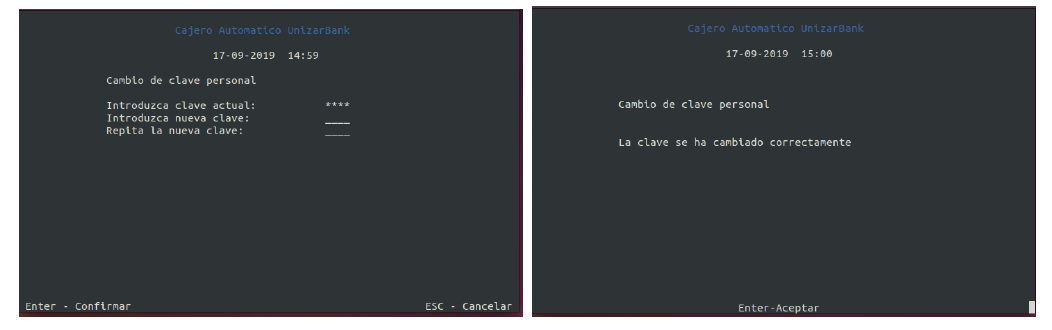
\includegraphics[scale=0.75]{images/funcionalidad7.png}
\caption{Captura de pantalla de la funcionalidad 7 (cambiar clave).}
\label{fig:captura_funcion_7}
\end{figure}

Se va a proceder a programar el fichero restante a partir de las capturas de pantalla recuperadas. En estas podemos observar que se aceptan 3 campos, dos correspondientes a la nueva clave y un tercero correspondiente a la clave actual. \\
El funcionamiento de este programa es sobrescribir el fichero \emph{tarjetas.ubd} para cambiar la clave de la tarjeta y el fichero \emph{intentos.ubd} para reiniciar los intentos fallidos de acceso a la tarjeta que se está cambiando el PIN.

\section{Parte 2: Nueva funcionalidad}

Esta tarea consiste en añadir una nueva funcionalidad al menú que consiste en mostrar todas las transferencias. Para esto, se ha requerido la modificación del funcionamiento de las transferencias, añadiendo la funcionalidad de realizar una transferencia programada, ya sea en una fecha específica o de manera mensual.\\
Para modificar el menú, se ha añadido un nuevo \emph{CHOICE}, con el fin de que el usuario pueda escoger la opción de listar transferencias, desplazando las otras dos funcionalidades como se ha propuesto en el enunciado.

\newpage
\begin{lstlisting}
	   IF CHOICE = 6 
               CALL "BANK9" USING TNUM
               GO TO PMENU.

           IF CHOICE = 7
               CALL "BANK7" USING TNUM
               GO TO PMENU.

           IF CHOICE = 8
               CALL "BANK8" USING TNUM
               GO TO PMENU.
\end{lstlisting}

En \emph{BANK9}, se ha seguido el esquema propuesto en \emph{BANK3} (consultar movimientos).
Para obtener únicamente las transferencias se ha modificado el filtrado y se ha tenido en cuenta el concepto del movimiento con el fin de saber si se debía mostrar. De esta manera también se permite obtener las transferencias programadas.


\begin{lstlisting}
IF MOV-CONCEPTO IS EQUAL TO "Transferimos" 
               OR MOV-CONCEPTO IS EQUAL TO "Nos transfieren"
               OR MOV-CONCEPTO IS EQUAL TO "Transferencia programada"
                   MOVE 1 TO MOV-VALIDO
           ELSE 
               MOVE 0 TO MOV-VALIDO. 
\end{lstlisting}

Para añadir la funcionalidad de las transferencias programadas se ha modificado el fichero \textit{BANK6.cbl} para permitir la inserción de la fecha a la que se programa la transferencia e indicar si es mensual. Si el campo fecha y mensual es vacío, se ejecuta una transferencia corriente. En caso contrario, se añade al fichero "programadas.ubd" un registro con la información relacionada con la transferencia programada. También se ha creado un nuevo fichero \emph{PROG.cbl} el cual es llamado desde el menú principal con la sentencia '\emph{CALL "PROG".}'. Cada vez que se ejecuta, comprueba el contenido del fichero "programadas.ubd", en el que se almacenan las transferencias programadas que no han sido ejecutadas. Si la fecha de uno de los registros del fichero es menor o igual a la actual en el momento que se lee, se debe de realizar la transferencia. El proceso que se lleva a cabo para ello es el mismo que proporciona las transferencias "normales". Adicionalmente, se comprueba el saldo de la cuenta origen en ese momento. \par
En caso de que la transferencia esté marcada como mensual, se debe modificar la fecha del registro correspondiente para que sea ejecutada en el siguiente mes. En caso contrario, tras realizar la transferencia, se elimina el registro correspondiente del archivo "programadas.ubd" y se continúa con la búsqueda de transferencias programadas. \par
Al mismo tiempo que se hace efectiva la transferencia, se deben añadir los registros de movimientos de la cuenta origen y destino, modificando el archivo "movimientos.ubd"

\section{Parte 3: Cambios en la aplicación}

\subsection{Mejorar la interfaz de usuario de ingresar efectivo}

En esta parte se pide modificar la forma de entrada de efectivo en el programa. Se debe admitir la introducción de billetes de 10, 20 y 50 euros.\\
Para realizar este comportamiento se debe modificar la entrada de texto y en lugar de admitir un número entero y un número que representa la parte decimal se admitirán 3 números naturales, correspondientes a las cantidades de los distintos billetes.\\

También se ha modificado la lógica del programa para hacer el cálculo del dinero en función de los billetes introducidos en el programa.\\

\begin{figure}[h!]
\centering
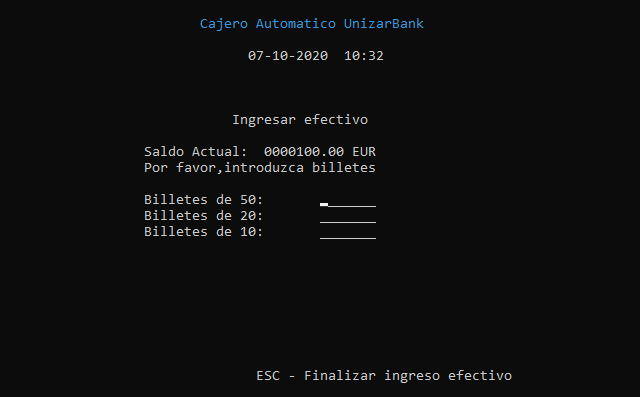
\includegraphics[scale=0.75]{images/pantalla_ingreso.png}
\caption{Captura de pantalla de la nueva interfaz de ingresar dinero.}
\label{fig:pantalla_ingreso}
\end{figure}

\newpage
\subsection{Mejorar la lectura de los mensajes}

En esta sección se pide cambiar los colores de los mensajes para facilitar la lectura de los mismos. En el caso de los mensajes que se presentan en fondo rojo se deberán mostrar en color blanco y los títulos deben tener un color más claro.\\

Para ello se buscarán los mensajes en los que haya ocurrencia de fondo rojo y se sustituirá el color de texto (\emph{FOREGROUND-COLOR}) de la siguiente forma:

\begin{lstlisting}
*> Antes
DISPLAY "Los codigos PIN nuevos no coinciden." 
               AT LINE 9 COL 26
               WITH FOREGROUND-COLOR IS BLACK
                    BACKGROUND-COLOR IS RED.
*> Despues
DISPLAY "Los codigos PIN nuevos no coinciden." 
               AT LINE 9 COL 26
               WITH FOREGROUND-COLOR IS WHITE
                    BACKGROUND-COLOR IS RED.
\end{lstlisting}

En el caso del título se buscarán todas las zonas en las que aparezca y se sustituirá el color azul por uno más claro (\emph{CYAN}):

\begin{lstlisting}
*> Antes
DISPLAY "Cajero Automatico UnizarBank" AT LINE 2 COL 26
               WITH FOREGROUND-COLOR IS BLUE.

*> Despues
DISPLAY "Cajero Automatico UnizarBank" AT LINE 2 COL 26
               WITH FOREGROUND-COLOR IS CYAN.
\end{lstlisting}


\begin{figure}[h!]
\centering
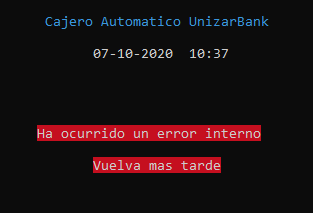
\includegraphics[scale=0.75]{images/error.png}
\caption{Captura de pantalla de la nueva interfaz del código de error.}
\label{fig:error}
\end{figure}

\subsection{Eliminar los ceros de la esquina inferior derecha}

En algunas pantallas aparecen ceros en la esquina inferior derecha. Esto se debe a que el programa está esperando la interacción del usuario en esa zona. Para evitar que aparezcan se debe buscar la variable que está esperando la entrada y añadirle el modificador \texttt{BLANK WHEN ZERO}. De esta manera ya no aparecerán los ceros.\\

\begin{figure}[h!]
\centering
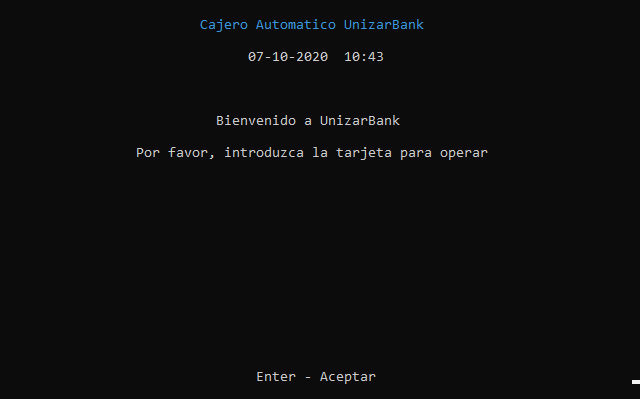
\includegraphics[scale=0.75]{images/ceros.png}
\caption{Captura de pantalla de la interfaz sin la aparición de ceros en la esquina inferior derecha.}
\label{fig:error}
\end{figure}

\newpage
\subsection{Ventana de ejecución de 80x25 caracteres}

Se pide que la ventana de ejecución tenga un tamaño dado. Esto tiene implicaciones directas en el código ya que en \emph{COBOL} es necesario establecer la línea y columna donde se va a mostrar un texto y por lo tanto no pueden excederse estos límites.\\
Para cumplir esta parte se ha comprobado que todas las líneas se encuentran entre 0 y 24 y que todas las columnas se encuentran entre 0 y 79.\\
\\
En la opción de \emph{Comprar entradas de espectáculos} se puede observar que si no se tiene en cuenta esta restricción el texto de las opciones de ventas aparece más allá de los límites de la pantalla. Esto se puede arreglar eliminando el \texttt{AT LINE 24 COL 80} de la línea en la que se aceptan los parámetros de entrada.

\end{document}